\documentclass[Research_Module_ES.tex]{subfiles}
\begin{document}
\section{Simulations}
After the evaluation of the asymptotic properties of the different \textit{Cross-Validation} procedures we want to take a closer look to the finite sample performance. Therefore, we consider the following model:
\[
	y_i=\beta_1+x_{2i}\beta_2+x_{3i}\beta_3+x_{4i}\beta_4+x_{5i}\beta_5+\varepsilon_i
\]
where $i=1,\ldots,n$ with $n$ being the total number of observations. The error terms $\varepsilon_i$ are iid form $N(01)$,  $x_{ki}$ is the i'th value of the k'th regression variable and all $x_{ki}$, $k=1,\ldots5$, are generated from different normal distributions\footnote{See Appendix}. Moreover, we assume that
\[
	\beta=(\beta_1,\beta_2,0,0,0)^\prime
\]
where $\beta_1,\beta_2$ are unequal to zero. So the Model with the best predictive ability have to be chosen out of five prossible regressor $\{x_1,\ldots,x_5\}$. \\
\\
For the different simulations we consider the five model section methods: CV(1), MCCV($n_\nu$),BICV($n_\nu$) and since they are popular in praxis AIC,BIC as benchmark. Also note that $n_v=n-\lfloor n^{3/4}\rfloor$.

\subsection{Ability of distinguishing between Category I and II }
In the first simulation we want to take a closer look at the probability given in Theorem (\ref{THM_Consistency of $CV(1)$} ) III. We saw that for $n\to\infty$ the different \textit{Cross-Validation} methods are perfectly able to distinguish between category I and II, hence the probability of choosing a model from Category I equals zero. But how god will \textit{Cross-Validation} perform with only finite information and will all methods behave similar?\\
\\
Figure \ref{Simulation1} shows how the probability of choosing a Category II model behaves for different sample sizes. To calculate these probabilities we repeat the procedure of model selection 2000 times for each sample size and plot the relative frequencies.\footnote{Note that for each of the 200 iterations a completely new sample was generated.}

As we can see in Figure \ref{Simulation1} the probabilities of choosing a Category II model is converging to 1 for all five methods. Moreover all methods perform quite similar in distinguishing between the two models only, the MCCV seems to be slightly worse then the over ones. The purpose of this is the smaller trainings set of MCCV which is chosen with $\lfloor n^{3/4}\rfloor$. Therefore MCCV only predicts $\Gamma_{\alpha,n-n_v}$, which is a less accurate estimate than $\Gamma_{\alpha,n}$ which is calculated by the other methods. 
\begin{figure}[h]
	\label{Simulation1}
	\centering
	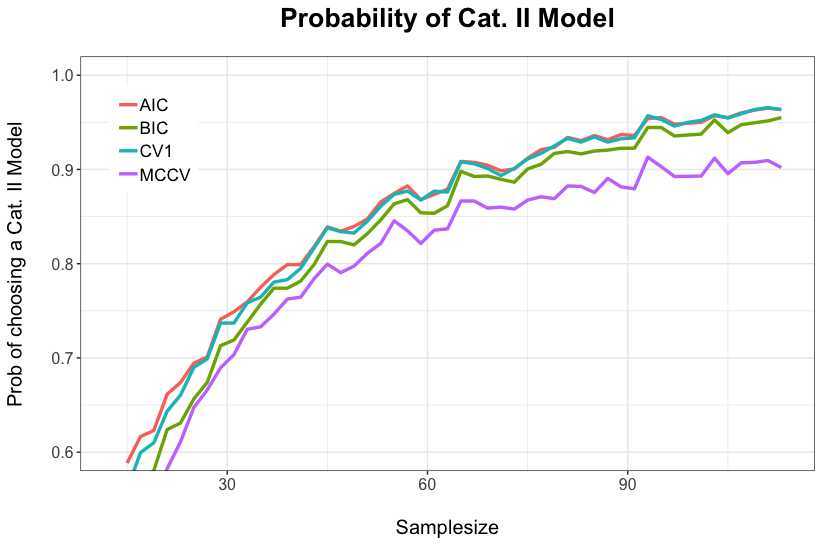
\includegraphics[width=1\textwidth]{Simulation1.png}\\
\caption{Probability of Choosing Cat II Models}
\end{figure}
\section{Ability of distinguishing in between Category II Models}




























\subsection{CV(1) and MCCV($n_{\nu}$)}
%BEISPIELTABELLE habe mal ein paar willkürliche sachen in der ersten zeile eingegeben, die wir später einfach nur ersetzen müssen, die letzten zeilen hab ich jetzt nicht weiter mit beispielzahlen gefüllt (ist noch eine alte tabelle von mir)
\begin{table}[htb]
	\begin{tabular}{lcccccc}
		\toprule
		\midrule
		\textbf{\scriptsize Initial $\beta$}
		&\textbf{\scriptsize Model $\mathcal{M}_\alpha$}&\textbf{\scriptsize Category}
		&\textbf{\scriptsize CV(1)}
		&\textbf{\scriptsize MCCV($n_\nu$)}
		&\textbf{\scriptsize APCV($n_\nu$)}
		&\textbf{\scriptsize BICV($n_\nu$)}\\
		$~$ &\textbf{\scriptsize $\alpha=\{...\}$} 
		\\\midrule\midrule
		
		{\scriptsize $\beta=(1,2,3,4,5,6)^\prime$}& \scriptsize alpha-werte & \scriptsize eins-oder-zwei &\scriptsize WertSpalte1 & \scriptsize WertSpalte2 &\scriptsize WertSpalte3 & \scriptsize WertSpalte4\\
		
		~& \scriptsize alpha-werte & \scriptsize eins-oder-zwei &\scriptsize WertSpalte1 & \scriptsize WertSpalte2 &\scriptsize WertSpalte3 & \scriptsize WertSpalte4\\
		
		~& \scriptsize alpha-werte &\scriptsize eins-oder-zwei & \scriptsize WertSpalte1 &\scriptsize WertSpalte2 & \scriptsize WertSpalte3 &\scriptsize WertSpalte4\\
		& & & & & &\\
		
		%ALTE tabelle
		{\scriptsize Initialset $\{X_{1},X_{2},X_{3},X_{4}\}$}\\
		{\scriptsize I-Score vor der Verwerfung}& \scriptsize 3,6896 & \scriptsize 7,1186 &\scriptsize 13,1224 & \scriptsize 14,2844 & & \\
		\scriptsize Verworfene Variable& \scriptsize $X_{3}$ &\scriptsize $X_{1}$ & \scriptsize $X_{2}$ &\scriptsize $X_{4}$ & & \\
		& & & & & &\\
		{\scriptsize Initialset $\{X_{1},X_{2},X_{3},X_{6}\}$}\\
		{\scriptsize I-Score vor der Verwerfung}& \scriptsize 2,0536 & \scriptsize 2,7195 &\scriptsize 3,9136 & \scriptsize 6,9534 & & \\
		\scriptsize Verworfene Variable& \scriptsize $X_{3}$ &\scriptsize $X_{6}$ & \scriptsize $X_{1}$ &\scriptsize $X_{2}$ & & \\
		& & & & & &\\
		{\scriptsize Initialset $\{X_{1},X_{3},X_{6}\}$}\\
		{\scriptsize I-Score vor der Verwerfung}& \scriptsize 0,8767 & \scriptsize 0,8681 &\scriptsize 0,1324 & & & \\
		\scriptsize Verworfene Variable& \scriptsize $X_{1}$ &\scriptsize $X_{6}$ & \scriptsize $X_{3}$ & & & \\
		\bottomrule
	\end{tabular}
	\caption{Verwerfungsprozess für vier Fälle}
\end{table}

\subsection{Different $n_{\nu}$}


\subsection{Consistency}

\subsection{Category \RM{1} - Simulation}


\end{document}